\chapter{Diseño e implementación}

\label{Chapter3}

Este capítulo detalla la arquitectura del prototipo de telemetría, el diseño del hardware, la implementación de la comunicación con los periféricos y la integración con el dispositivo móvil.

El capítulo se organiza en cinco ejes alineados con la estructura del proyecto. Primero se describe la arquitectura del sistema y el uso de la memoria del integrado. Segundo se presenta el diseño del hardware del prototipo. Tercero se documenta el diseño del firmware embebido y sus módulos principales. Cuarto se describen las interfaces de comunicación y el formato de los mensajes intercambiados. Quinto se explica la integración con la aplicación web en el teléfono.

%----------------------------------------------------------------------------------------
\section{Arquitectura del sistema}
\label{sec:arquitectura-sistema}

El sistema se dividió en dos partes con acoplamiento flexible. El dispositivo embebido en la motocicleta adquirió datos inerciales y de posicionamiento, registró series temporales en almacenamiento local y expuso un enlace serie hacia un módulo BLE. El teléfono móvil concentró la interfaz de usuario, la visualización cartográfica y la recepción de telemetría cuando existió emparejamiento inalámbrico. Esa separación preservó el registro autónomo aun si el conductor no abrió la aplicación web.

\subsection{Interconexión de módulos}

En la placa NUCLEO-F446RE se centralizó la lectura de sensores, el acceso a la tarjeta microSD y el uso de tres instancias USART. El receptor NEO-M8N entregó tramas NMEA por USART1. La unidad inercial LSM6DSO respondió por I2C1. El módulo HC-10 reenvió octetos entre el integrado y el controlador Bluetooth del teléfono. En la figura~\ref{fig:interconexion-buses-cap3} se resume la asignación lógica entre los bloques de hardware.

\begin{figure}[H]
	\centering
	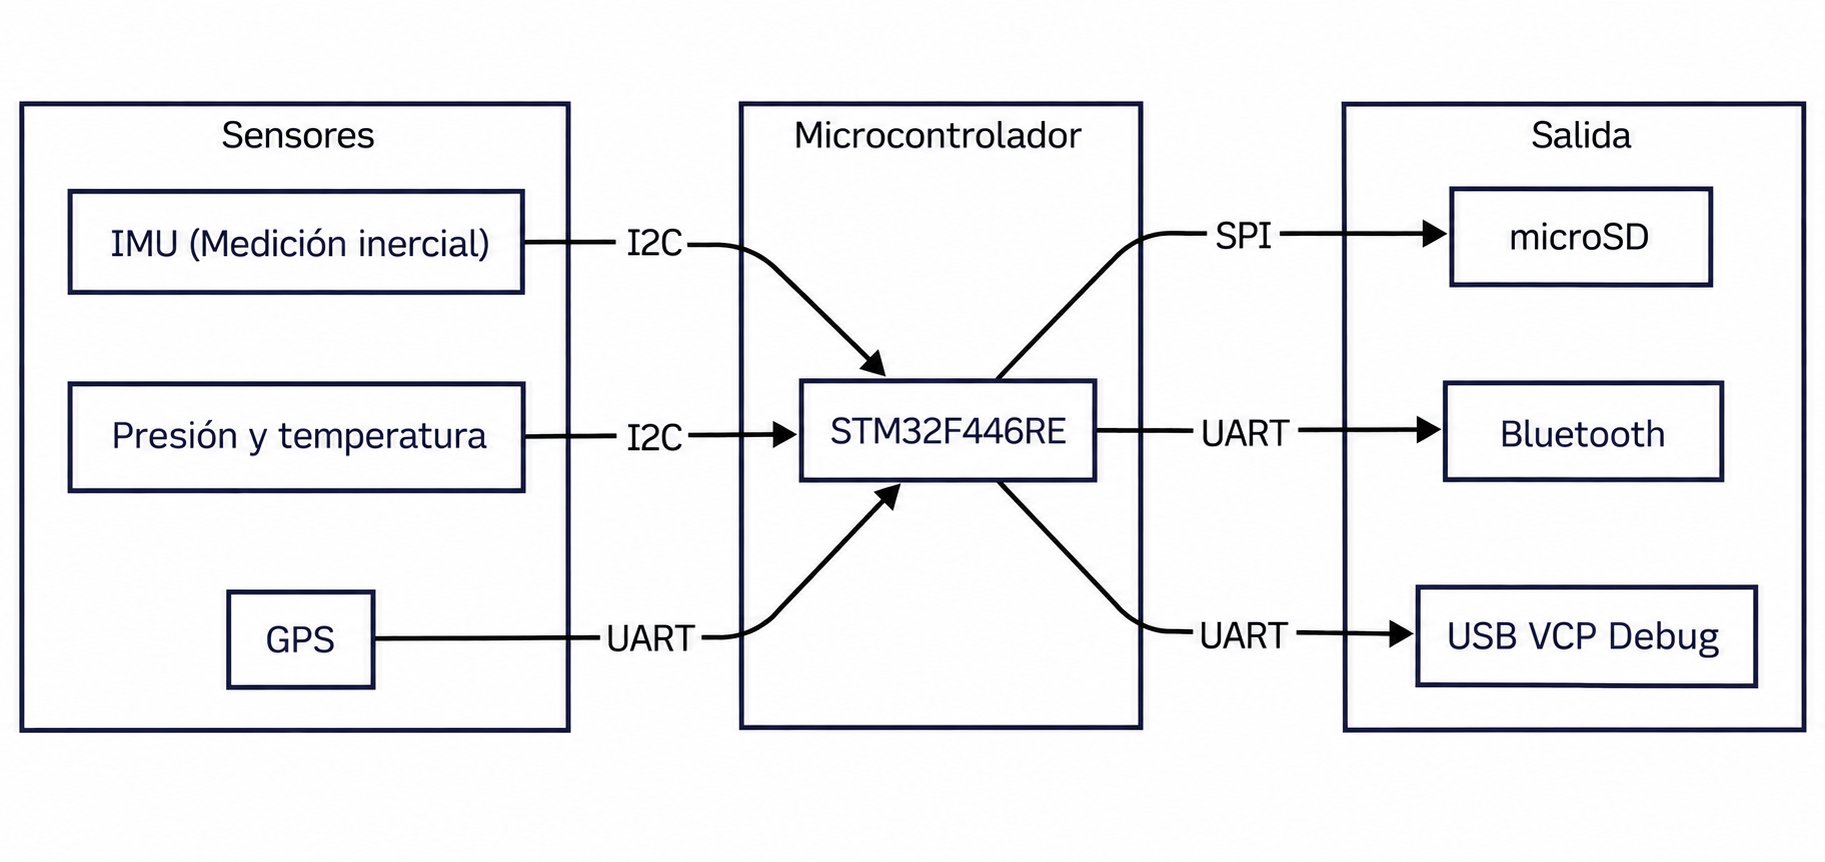
\includegraphics[width=0.92\textwidth]{Figures/interconexion-buses.png}
	\caption[Arquitectura en bloques]{Diagrama en bloques de la interconexión entre el microcontrolador y los periféricos del prototipo.}
	\label{fig:interconexion-buses-cap3}
\end{figure}

\subsection{Arquitectura de software}

En el microcontrolador intervinieron la capa HAL, controladores para GNSS, unidad inercial, enlace Bluetooth y registro en tarjeta microSD, además del middleware FatFs \citep{chan_fatfs}. Sobre esa base se empleó el sistema operativo de tiempo real FreeRTOS \citep{freertos}. Esa capa habilitó ejecutar en paralelo la adquisición de sensores, el registro en microSD y la publicación por Bluetooth, asignar prioridades distintas a cada actividad y coordinar el acceso compartido mediante colas, semáforos y exclusión mutua. A partir de ese esquema, la aplicación embebida se organizó en tareas concurrentes. El acceso al hardware quedó mediado por drivers y por transferencias DMA en los enlaces de mayor caudal. En el teléfono, la PWA usó el Bluetooth del navegador \citep{mdn_pwa}\citep{w3c_web_bluetooth} para conectarse al dispositivo embebido y recibir telemetría. En la figura~\ref{fig:capas-software-cap3} se contrastan ambos lados del sistema.

\begin{figure}[H]
	\centering
	\includegraphics[width=0.95\textwidth]{Figures/cap2-capas-software.png}
	\caption[Capas de software]{Capas de software en el microcontrolador y en el teléfono móvil.}
	\label{fig:capas-software-cap3}
\end{figure}

\subsection{Uso de la memoria del integrado}
\label{sec:modelo-memoria-mcu}

El código del firmware residió en la memoria flash interna. En la SRAM se ubicaron las pilas de las tareas del RTOS, los buffers de DMA, las colas de mensajes y las estructuras de telemetría. No se utilizó una memoria de programa externa. La descripción de pines, relojes, instancias de DMA y periféricos se generó con STM32CubeMX y se integró al proyecto en STM32CubeIDE \citep{st_stm32cubeide}. El IWDG se habilitó como una supervisión ante bloqueos del software y se alimentó de forma periódica desde una tarea dedicada del RTOS.

%----------------------------------------------------------------------------------------
\section{Diseño del hardware}
\label{sec:diseno-hardware}

En esta sección se describe el esquema eléctrico, el diseño del circuito impreso y la interconexión de los bloques de hardware del prototipo.

\subsection{Esquema eléctrico}

El esquema reunió el microcontrolador, la alimentación, los conectores hacia GNSS, la unidad inercial, la tarjeta microSD y el módulo de enlace Bluetooth, con la misma asignación lógica de buses que en la figura~\ref{fig:interconexion-buses-cap3}. En la figura~\ref{fig:cap3-esquema-electrico} se muestra el diagrama eléctrico del prototipo.

\begin{figure}[H]
	\centering
	\fbox{\begin{minipage}{0.9\textwidth}
		\centering\vspace{0.28\textheight}
		\textit{Espacio reservado para el esquema eléctrico.}\vspace{0.28\textheight}
	\end{minipage}}
	\caption[Esquema eléctrico]{Esquema eléctrico del prototipo de telemetría.}
	\label{fig:cap3-esquema-electrico}
\end{figure}

\subsection{Circuito impreso}

El circuito impreso integró los bloques del esquema en un único PCB orientado al montaje en el vehículo. En la figura~\ref{fig:cap3-pcb} se presenta el diseño de la placa (vista superior o de ensamblado).

\begin{figure}[H]
	\centering
	\fbox{\begin{minipage}{0.9\textwidth}
		\centering\vspace{0.28\textheight}
		\textit{Espacio reservado para el diseño del circuito impreso.}\vspace{0.28\textheight}
	\end{minipage}}
	\caption[Circuito impreso]{Vista del circuito impreso del prototipo.}
	\label{fig:cap3-pcb}
\end{figure}

%----------------------------------------------------------------------------------------
\section{Diseño del firmware}
\label{sec:diseno-firmware}

\subsection{Organización en módulos}

La lógica embebida se repartió en controladores que encapsulan cada periférico y en tareas de FreeRTOS que orquestan el muestreo y la publicación de datos. Los módulos \texttt{gps} y \texttt{lsm6dso} abstraen la lectura de GNSS y de la IMU. El módulo \texttt{bt\_module} concentra el envío por USART3. El módulo \texttt{sd\_logger}, junto con FatFs, administra el fichero CSV en la tarjeta microSD.

Tras la inicialización del hardware y el arranque del planificador del sistema operativo, coexistieron tareas de adquisición y análisis de NMEA, lectura periódica de la IMU, registro en la tarjeta microSD, enlace Bluetooth y supervisión con IWDG. Las tareas que acceden al bus SPI de la tarjeta serializaron el acceso al medio mediante un mutex (del inglés \textit{mutual exclusion}) del RTOS para evitar corrupción de ficheros. Los eventos entre módulos se canalizaron con colas y temporizadores de software del kernel. En la figura~\ref{fig:cap3-flujo-firmware} se resume el reparto entre tareas y el flujo de datos hasta la publicación por Bluetooth.

\begin{figure}[H]
	\centering
	\fbox{\begin{minipage}{0.88\textwidth}
		\centering\vspace{0.32\textheight}
		\textit{Espacio reservado para diagrama de flujo del firmware.}\vspace{0.32\textheight}
	\end{minipage}}
	\caption[Flujo del firmware]{Diagrama de tareas del RTOS y flujo de telemetría.}
	\label{fig:cap3-flujo-firmware}
\end{figure}

%----------------------------------------------------------------------------------------
\section{Comunicaciones e interfaces}
\label{sec:comunicaciones-implementacion}

\subsection{Asignación de periféricos}

En el STM32F446RE se configuró qué instancia de cada bus (USART, I2C y SPI) enlazó a cada módulo del prototipo, con pines y velocidad definidos en STM32CubeMX. La tabla~\ref{tab:parametros-buses} resume esa asignación, el modo de operación y el rol de cada enlace en el firmware.

\begin{table}[H]
	\centering
	\caption[Parámetros de buses]{Parámetros de los buses configurados en el prototipo.}
	\setlength{\tabcolsep}{4pt}
	\begin{tabularx}{\textwidth}{@{}>{\raggedright\arraybackslash}p{1.45cm}>{\raggedright\arraybackslash}p{1.95cm}>{\raggedright\arraybackslash}p{2.35cm}>{\raggedright\arraybackslash}X@{}}
		\toprule
		\textbf{Bus} & \textbf{Periférico} & \textbf{Tasa / modo} & \textbf{Rol en el sistema} \\
		\midrule
		USART1 & NEO-M8N & 9600 baudios & Recepción NMEA por DMA hacia buffer circular \\
		USART2 & ST-LINK VCP & 115200 baudios & Consola de depuración hacia el host \\
		USART3 & HC-10 (BLE) & 9600 baudios & Enlace serie transparente con el teléfono \\
		I2C1 & LSM6DSO & 100kHz, maestro & Lectura periódica de registros de la IMU \\
		SPI2 & microSD & Maestro, DMA & Almacenamiento de ficheros CSV mediante FatFs \\
		\bottomrule
	\end{tabularx}
	\label{tab:parametros-buses}
\end{table}

\subsection{Protocolo de telemetría sobre el enlace serie}
\label{sec:protocolo-telemetria-serie}

En USART1 el canal DMA trasladó los octetos entrantes a un buffer circular. Una tarea de mayor prioridad reconstruyó las sentencias NMEA \citep{nmea_0183} a partir de ese buffer y, si una línea era válida, se conservó en memoria la posición, la hora y los demás datos de navegación que aportaba. Las líneas incompletas o incorrectas se descartaron. En I2C1 la unidad inercial se consultó en modo maestro a 100kHz con dirección de 7 bits 0x6A desde la tarea de adquisición.

En USART3 el módulo HC-10 funcionó como túnel serie hacia el teléfono. El microcontrolador envió octetos por UART y el módulo los reexpuso por BLE para que el navegador móvil los recibiera. Una tarea de enlace publicó la telemetría en formato JSON. Los mensajes inerciales aportaron aceleraciones y velocidades angulares en los tres ejes, junto con la temperatura de la unidad, con magnitudes representadas como enteros escalados. Los mensajes de posicionamiento indicaron el tipo de fijación GNSS, derivado de las sentencias NMEA: sin posición, fijación en dos dimensiones, fijación en tres dimensiones con altitud o fijación con corrección diferencial. También incluyeron coordenadas geográficas, altitud, velocidad sobre el suelo, cantidad de satélites en uso y rumbo. No se definió un protocolo binario propietario sobre el UART.

En SPI2 las transferencias en bloque hacia la tarjeta se realizaron con DMA bajo FatFs para reducir la carga del núcleo durante la escritura del fichero CSV. Cada registro incluyó una marca temporal en milisegundos, la hora UTC cuando el receptor GNSS dispuso de fecha y hora válidas, las tres componentes de aceleración y de velocidad angular, y la temperatura de la IMU. La primera fila del archivo declaró las columnas correspondientes y las sucesivas se alinearon al período de muestreo configurado en el firmware.

En la figura~\ref{fig:cap3-formato-mensaje} se representa la organización de los mensajes JSON. En la figura~\ref{fig:cap3-secuencia-comunicacion} se ilustra la secuencia entre el ciclo de telemetría, el módulo HC-10 y el dispositivo móvil.

\begin{figure}[H]
	\centering
	\fbox{\begin{minipage}{0.88\textwidth}
		\centering\vspace{0.22\textheight}
		\textit{Espacio reservado para organización de la trama o del mensaje JSON.}\vspace{0.22\textheight}
	\end{minipage}}
	\caption[Organización del mensaje]{Organización de los campos en los mensajes JSON de telemetría.}
	\label{fig:cap3-formato-mensaje}
\end{figure}

\begin{figure}[H]
	\centering
	\fbox{\begin{minipage}{0.88\textwidth}
		\centering\vspace{0.30\textheight}
		\textit{Espacio reservado para diagrama de secuencia de comunicación.}\vspace{0.30\textheight}
	\end{minipage}}
	\caption[Secuencia de comunicación]{Diagrama de secuencia del intercambio entre firmware, HC-10 y dispositivo móvil.}
	\label{fig:cap3-secuencia-comunicacion}
\end{figure}

\subsection{Canal de depuración}

USART2 se asignó al puerto virtual del depurador ST-LINK. A 115200 baudios se emitieron mensajes periódicos con lecturas de sensores, estado de la tarjeta y del enlace Bluetooth. Ese canal no alimentó la aplicación del usuario, pero apoyó la verificación del prototipo durante el desarrollo. La emisión de esas trazas quedó prevista como desactivable al compilar el firmware, de modo que la versión orientada al uso productivo pudiera prescindir de ellas sin alterar la telemetría JSON por BLE ni el registro en microSD.

%----------------------------------------------------------------------------------------
\section{Integración entre hardware y software}
\label{sec:integracion-hw-sw}

\subsection{Dispositivo móvil}

La interfaz del usuario se implementó como PWA con React \citep{react} y Vite \citep{vite}, accesible desde el navegador sin publicar un binario en las tiendas de aplicaciones. La capa de presentación accedió al HC-10 mediante Web Bluetooth y al perfil GATT (del inglés \textit{Generic Attribute Profile}) del CC2541. Los mapas emplearon Leaflet \citep{leaflet} para situar en un plano la posición GNSS recibida y dibujar el recorrido a medida que llegaban nuevos puntos. El análisis de la telemetría se ejecutó en el navegador del dispositivo móvil y liberó carga de procesamiento en el microcontrolador.

\subsection{Flujo de datos extremo a extremo}

El registro local en CSV sobre microSD conservó series temporales cuando el teléfono no estaba emparejado. El intercambio inalámbrico cubrió la visualización en tiempo casi real y la consulta del estado del dispositivo según el período de telemetría definido en las tareas del firmware. En la figura~\ref{fig:cap3-integracion-e2e} se resume la adquisición, la escritura en tarjeta y el envío por Bluetooth en un diagrama de integración extremo a extremo.

\begin{figure}[H]
	\centering
	\fbox{\begin{minipage}{0.88\textwidth}
		\centering\vspace{0.30\textheight}
		\textit{Espacio reservado para diagrama de integración extremo a extremo.}\vspace{0.30\textheight}
	\end{minipage}}
	\caption[Integración extremo a extremo]{Flujo de datos entre sensores, almacenamiento local y dispositivo móvil.}
	\label{fig:cap3-integracion-e2e}
\end{figure}